\section{Light Attenuation}
Fits are done based on 2-strip pixels corresponding to strip number. 
The strip number is converted into distance by a process using equations \ref{eq:udist}-\ref{eq:wdist}, 
equation \ref{eq:s}, and an offset to have the distance quoted to the center of the physical bin. 
The exccess fiber lengths in theory could be added into the distance, but will only cause a shift in the fit.
The fiber lengths are taken from the PCAL geometry note \cite{bib:geomnote}. 
% and are listed in section \ref{sec:fiberlength}.
The Gaussian centroids can be found as a function of total distance from the edge of the PCAL unit.
This total distance is fit to an exponential form. 




\subsection{Strip Number vs Distance}
\FloatBarrier

The overlaid strip numbers convert directly into distance as seen by Figure \ref{fig:lowqualdist}

\begin{figure}[h]
\centering
\includegraphics[height= 3in, keepaspectratio = true]{lowqualitydiagram}
\caption{A cartoon schematic of the pcal unit demonstrates the method to correct for the light attenuation.}
\label{fig:lowqualdist}
\end{figure}


%\FloatBarrier
%\subsection{Fiber Length}
%\label{sec:fiberlength}
%Fiber lengths for each individual strip can be found in the PCAL geometry note \cite{bib:geomnote}.
%These table have been recorded and added into the calibration. 



\FloatBarrier
\subsection{Fit Function}
\FloatBarrier
The fit function suggested in the geometry note is an  exponential (equation \ref{eq:exp}).
It is also suggested that here the distance, $L$, should include the distance from the end of the strip 
to the cosmic ray track, $L_{s}$, as well as the extra fiber length, $L_{f}$.
In other words $L = L_{s} + L_{f}$.
However to analyze the quality of fit $L_{f}$ can be treated as a constant and absorbed into the parameter 
$a$ in equation \ref{eq:exp}.

\begin{equation}
    I = e^{a + bL}
    \label{eq:exp}
\end{equation}

\begin{figure}[h]
    \centering
    \begin{subfigure}[h]{0.4\textwidth}
        \includegraphics[width= \textwidth, keepaspectratio = true]{exponetial67}
        \caption{Shown is a fit with equation \ref{eq:exp}, where the y axis is the ADC value and the x axis is $L_{s}$.}
        \label{fig:exponential67}
    \end{subfigure}
    ~
    \begin{subfigure}[h]{0.4\textwidth}
        \includegraphics[width= \textwidth, keepaspectratio = true]{exponetialwfib67}
        \caption{Shown is a fit with equation \ref{eq:exp}, where the y axis is the ADC value and the x axis is $L_{s} + L_{f}$.}
        \label{fig:exponentialwfib67}
    \end{subfigure}
    \caption{Plotted is the fit of equation \ref{eq:exp}, where $L = L_{s}$ (a) and $L = L_{s} + L_{f}$ (b).}
    \label{fig:expfit}
\end{figure}

As seen by figure \ref{fig:expfit}, a single exponential may not be the best fit for the data.
One might suggest a fitting function similar to equation \ref{eq:try1}, in order to separate the fiber 
attenuation from the scintillator attenuation.
However this function again can reduce to equation \ref{eq:exp} because $L_{f}$ is a constant for each 
scintillator strip and is seen not to be a good fit.


\begin{equation}
    \begin{split}
        I &= a_{1}e^{b_{1}(L_{s} + L_{f})}e^{b_{2}L_{s}} \\
          &= a_{1}e^{b_{1}(L_{s} + L_{f}) + b_{2}L_{s}} \\
          &= a_{1}e^{(b_{1} + b_{2})L_{s} + b_{1}L_{f}} \\
          &= a_{1}e^{b_{1}L_{f}}e^{(b_{1} + b_{2})L_{s}} \\
          &= e^{a}e^{(b_{1} + b_{2})L_{s}} \\
          &= e^{a}e^{bL_{s}} \\
          &= e^{a + bL_{s}} \\
    \end{split}
    \label{eq:try1}
\end{equation}

\begin{comment}
\begin{equation}
    I(L_{s})= ae^{(b_{1} + b_{2})L_{s} + b_{1}L_{f}}
    \label{eq:try1mid}
\end{equation}

\FloatBarrier
\begin{figure}[h]
    \centering
    \includegraphics[width= 3in, keepaspectratio = true]{exponential67eq9}
    \caption{Plotted is the fit of equation \ref{eq:try1mid} as a function of $L_{s}$.}
    \label{fig:try1mid}
\end{figure}
\end{comment}
\FloatBarrier


Other functional forms that could represent the data should be similar to that of an exponential.
A couple of these forms include an exponential plus a constant or a sum of exponentials.
In both cases, some considerations have to be made on the domain of the function.
The sum of two exponentials was considered to have some portion of the attenuation in the fibers to 
be different than inside the scintillator. This does not get a better fit, and does not allow any more 
information to be extracted. Therefore the function used in fitting the attenuation was chosen to be 
an exponential with an added constant as seen by Equation \ref{eq:expplusconst}.

\begin{equation}
    I(L_{s}) = ae^{bL_{s}}+c
    \label{eq:expplusconst}
\end{equation}


\FloatBarrier
\subsection{Calibration Constants}
A table of constants can be uploaded to the clas12 database once the fitting procedure is complete.
%To get the calibration constants below, parameter limits were set on equation \ref{eq:expplusconst} 
%for $200.0 < a < 900.0$, $-0.009 < b < -0.0005$, and $0.0 < c < 700.0$, based on qualitative observation on a global fit.
On strips where less than five points were available for fitting, either 
a single exponential or a constant term was used for the fitting function. This was done to avoid situations 
with more parameters than points available. In general the less points available for the fit, the shorter 
the strip is, allowing for less of a need for a correction. All the fits shown are for Sector One of the PCAL.
\FloatBarrier
\vspace{5mm}

%Ufits:
\begin{figure}[h]
    \centering
    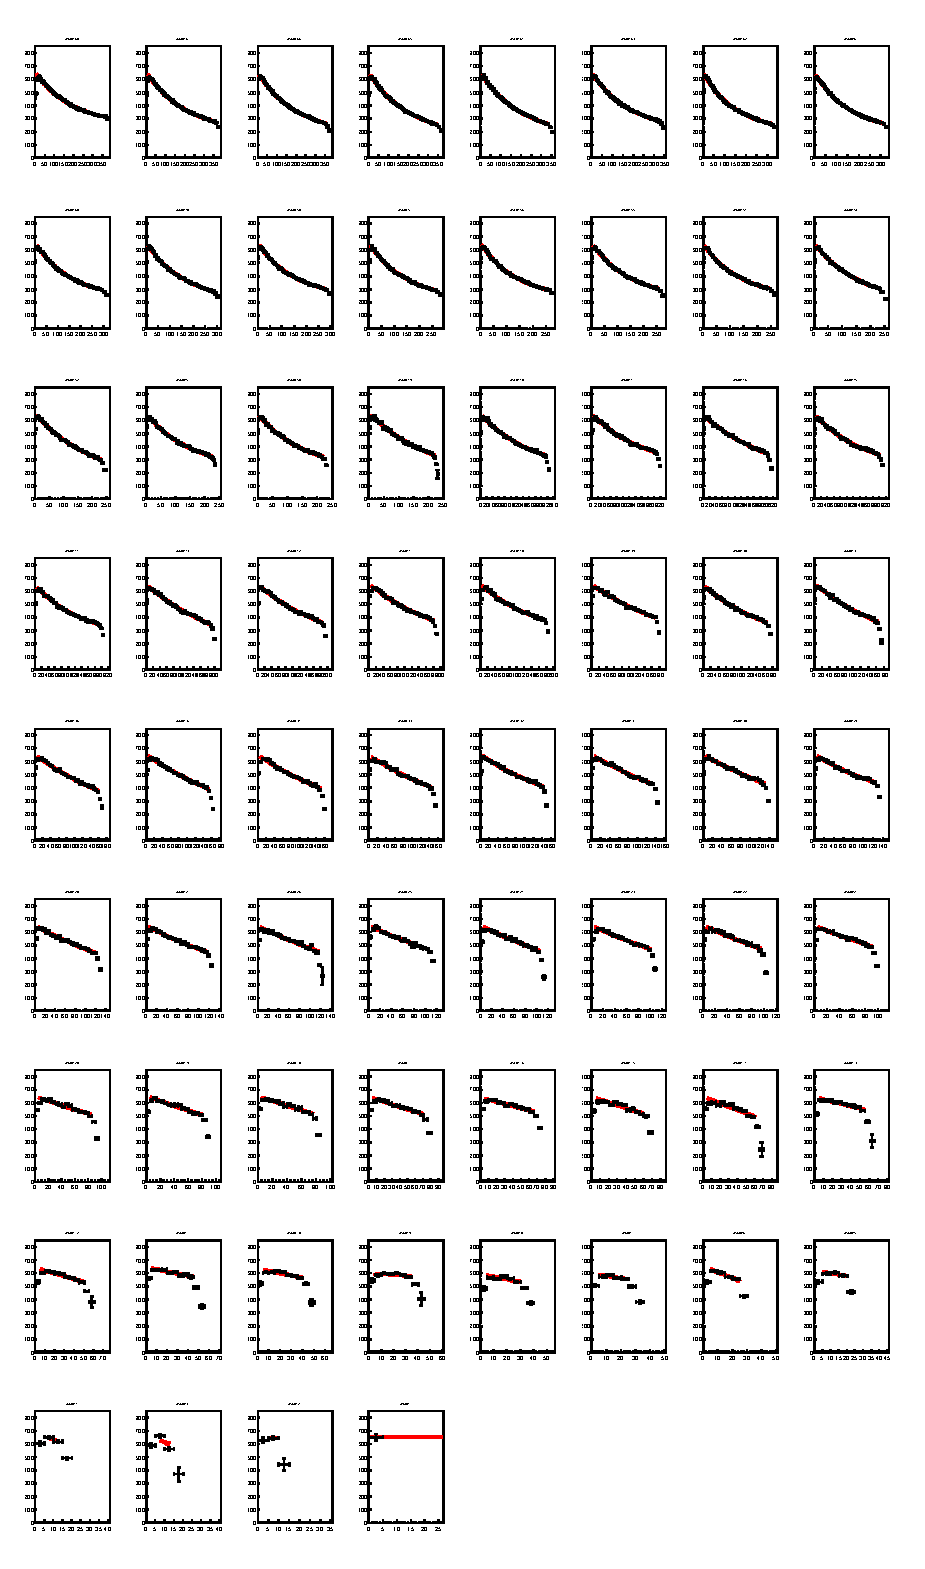
\includegraphics[width= 6.5in, height = 8in, keepaspectratio = true]{allustrips}
    \caption{Plotted are all of the u strip attenuation plots starting at 68 in the upper left hand corner. 
    These plots are all plotted on a linear scale. The y-axis is set from 0 to 850 and the x-axis varies 
    depending on the number of points in the plot.}
    \label{fig:allustrips}
\end{figure}

\FloatBarrier
%Vfits:
\begin{figure}[h]
    \centering
    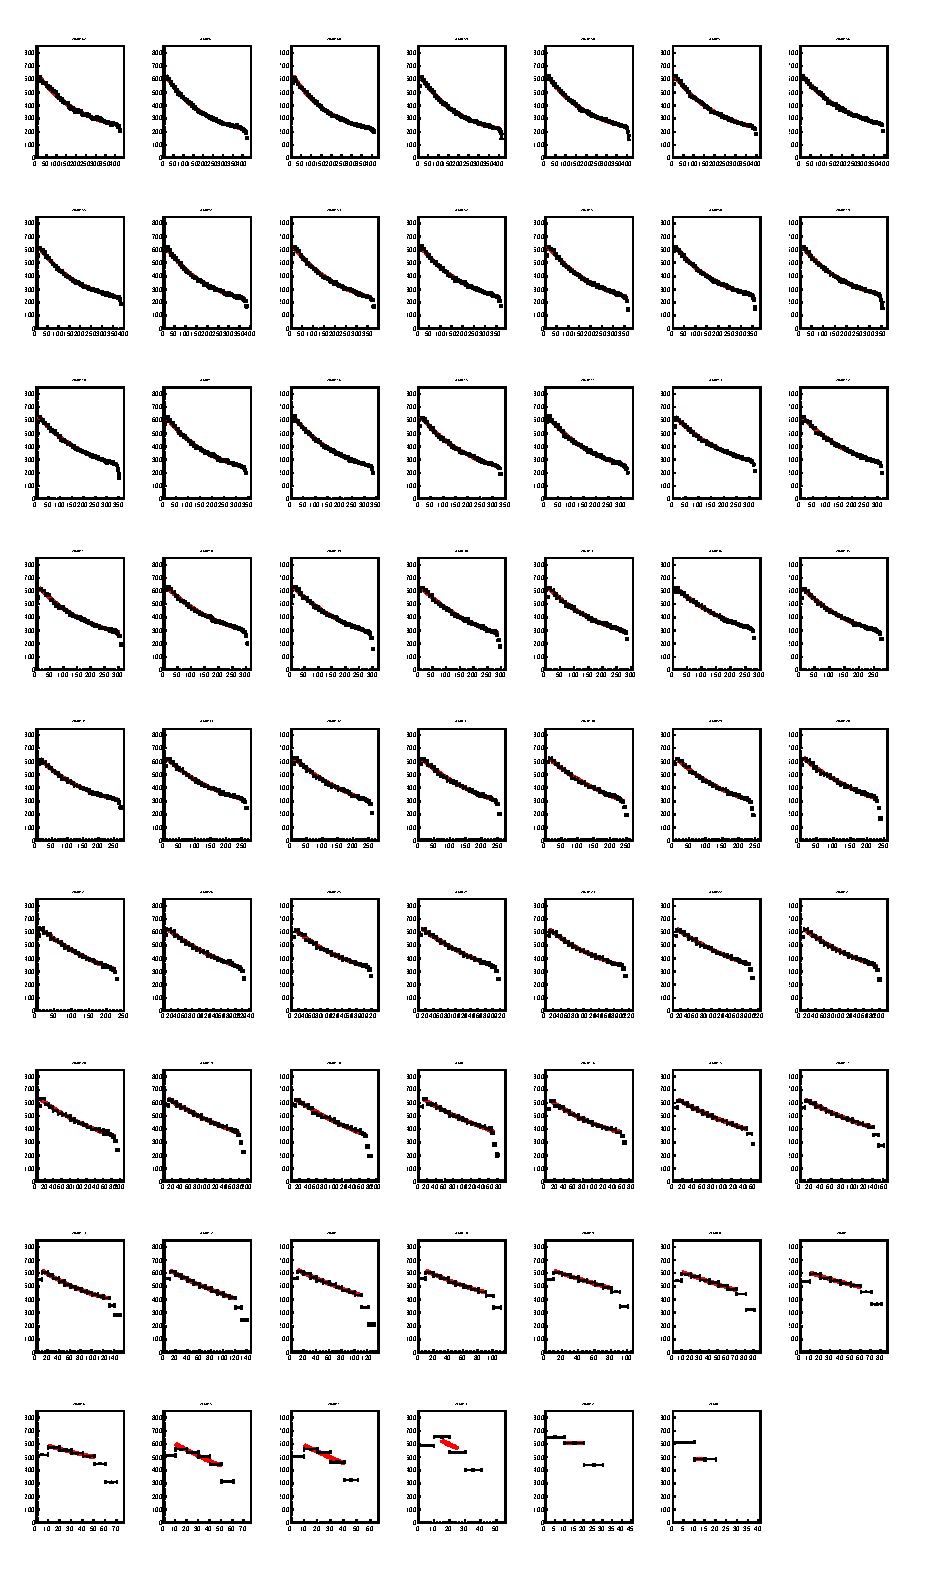
\includegraphics[width= 6.5in, height = 8in, keepaspectratio = true]{allvstrips}
    \caption{Plotted are all of the v strip attenuation plots starting at 62 in the upper left hand 
    corner. These plots are all plotted on a linear scale. The y-axis is set from 0 to 850 and the 
    x-axis varies depending on the number of points in the plot.}
    \label{fig:allvstrips}
\end{figure}


\FloatBarrier

%Wfits:
\begin{figure}[h]
    \centering
    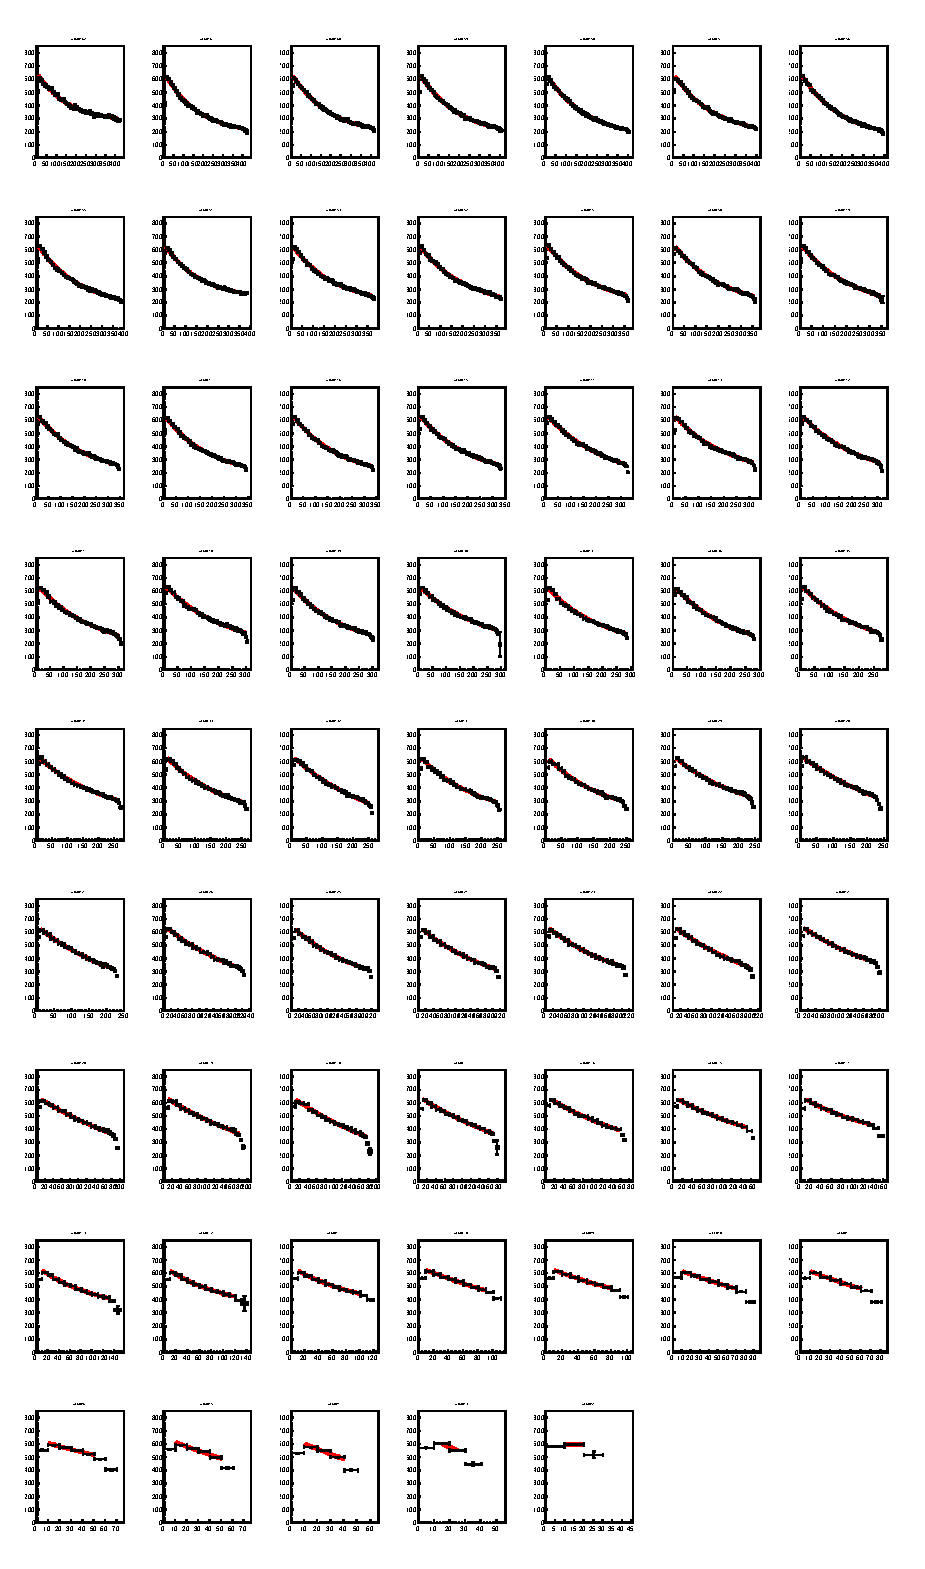
\includegraphics[width= 6.5in, height = 8in, keepaspectratio = true]{allwstrips}
    \caption{Plotted are all of the w strip attenuation plots starting at 62 in the upper left 
    hand corner. These plots are all plotted on a linear scale. The y-axis is set from 0 to 850 
    and the x-axis varies depending on the number of points in the plot.}
    \label{fig:allustrips}
\end{figure}

\FloatBarrier
\begin{table}[h]
        \centering{}
        \scalebox{0.75}{
        \begin{tabular}{|c|c|c|c|}
            \hline
            U-Strip &  Parameter $a$  &Parameter $b$  & Parameter $c$ \\ \hline
1   &   650   &   0   &   0  \\  \hline  
2   &   650   &   0   &   0  \\  \hline  
3   &   650   &   -0.009   &   0  \\  \hline  
4   &   650   &   -0.009   &   0  \\  \hline  
5   &   616.113   &   -0.00639717   &   33.8858  \\  \hline  
6   &   649.996   &   -0.00717551   &   0.0046356  \\  \hline  
7   &   649.968   &   -0.00318808   &   0.0319326  \\  \hline  
8   &   649.972   &   -0.00232476   &   0.0273016  \\  \hline  
9   &   649.146   &   -0.00112904   &   0.854413  \\  \hline  
10   &   649.999   &   -0.00281005   &   0.000286188  \\  \hline  
11   &   649.993   &   -0.00286292   &   0.00718601  \\  \hline  
12   &   650   &   -0.0041656   &   0.000445736  \\  \hline  
13   &   650   &   -0.003283   &   0.000103724  \\  \hline  
14   &   649.997   &   -0.00376077   &   5.37227e-06  \\  \hline  
15   &   650.001   &   -0.00339912   &   6.96689e-06  \\  \hline  
16   &   649.997   &   -0.00305411   &   8.14649e-06  \\  \hline  
17   &   649.999   &   -0.00345134   &   9.95183e-09  \\  \hline  
18   &   649.998   &   -0.00310718   &   4.19396e-07  \\  \hline  
19   &   650   &   -0.00311517   &   5.01049e-06  \\  \hline  
20   &   650   &   -0.00281725   &   6.09084e-06  \\  \hline  
21   &   650   &   -0.00315783   &   3.38135e-05  \\  \hline  
22   &   650   &   -0.00328681   &   2.55834e-08  \\  \hline  
23   &   650   &   -0.00316776   &   2.15877e-05  \\  \hline  
24   &   649.999   &   -0.00317021   &   4.66803e-05  \\  \hline  
25   &   650   &   -0.00327065   &   5.9556e-06  \\  \hline  
26   &   650.001   &   -0.00309179   &   1.40689e-08  \\  \hline  
27   &   551.087   &   -0.00385902   &   98.9141  \\  \hline  
28   &   649.997   &   -0.00307714   &   7.49416e-05  \\  \hline  
29   &   419.522   &   -0.00552754   &   230.477  \\  \hline  
30   &   650   &   -0.00316014   &   0.000130702  \\  \hline  
31   &   650.001   &   -0.00312815   &   2.25921e-06  \\  \hline  
32   &   585.658   &   -0.00373922   &   64.3455  \\  \hline  
33   &   581.001   &   -0.00374214   &   68.997  \\  \hline  
34   &   650.002   &   -0.00328878   &   0.000131253  \\  \hline  
35   &   650   &   -0.00332314   &   1.43305e-05  \\  \hline  
36   &   649.998   &   -0.00340294   &   1.07435e-07  \\  \hline  
37   &   556.399   &   -0.00428136   &   93.5991  \\  \hline  
38   &   483.854   &   -0.00534903   &   166.146  \\  \hline  
39   &   482.458   &   -0.00431684   &   167.541  \\  \hline  
40   &   392.765   &   -0.00669036   &   257.235  \\  \hline  
41   &   499.22   &   -0.00443664   &   150.78  \\  \hline  
42   &   513.839   &   -0.00445738   &   136.164  \\  \hline  
43   &   581.507   &   -0.00388427   &   68.4914  \\  \hline  
44   &   391.463   &   -0.00757633   &   258.536  \\  \hline  
45   &   434.393   &   -0.00632194   &   215.608  \\  \hline  
46   &   463.813   &   -0.00513914   &   186.187  \\  \hline  
47   &   413.809   &   -0.00605594   &   236.189  \\  \hline  
48   &   442.234   &   -0.00592955   &   207.766  \\  \hline  
49   &   509.976   &   -0.00449146   &   140.024  \\  \hline  
50   &   443.895   &   -0.00614484   &   206.105  \\  \hline  
51   &   425.765   &   -0.00641114   &   224.233  \\  \hline  
52   &   504.812   &   -0.00511618   &   145.188  \\  \hline  
53   &   454.838   &   -0.0061679   &   195.162  \\  \hline  
54   &   406.411   &   -0.00766326   &   243.589  \\  \hline  
55   &   415.976   &   -0.00690821   &   234.026  \\  \hline  
56   &   421.326   &   -0.00710769   &   228.675  \\  \hline  
57   &   435.635   &   -0.00660386   &   214.362  \\  \hline  
58   &   411.518   &   -0.00663318   &   238.483  \\  \hline  
59   &   438.882   &   -0.00625669   &   211.118  \\  \hline  
60   &   423.763   &   -0.00618908   &   226.238  \\  \hline  
61   &   444.671   &   -0.0063621   &   205.328  \\  \hline  
62   &   438.481   &   -0.00674885   &   211.519  \\  \hline  
63   &   437.138   &   -0.00564978   &   212.862  \\  \hline  
64   &   482.525   &   -0.00495599   &   167.473  \\  \hline  
65   &   473.388   &   -0.00516614   &   176.613  \\  \hline  
66   &   465.633   &   -0.00500512   &   184.367  \\  \hline  
67   &   455.941   &   -0.00479029   &   194.059  \\  \hline  
68   &   410.201   &   -0.00506009   &   239.798  \\  \hline  
        \end{tabular}
        }
        \caption{Calibration Constants for the U layer.}
        \label{tab:UattenC}
\end{table}


\begin{table}[h]
        \centering
        \scalebox{0.75}{
        \begin{tabular}{|c|c|c|c|}
            \hline
            V-Strip &  Parameter $a$  &Parameter $b$  & Parameter $c$ \\ \hline
1   &   650.002   &   0   &   0  \\  \hline  
2   &   649.999   &   0   &   0  \\  \hline  
3   &   650.001   &   -0.009   &   0  \\  \hline  
4   &   650.001   &   -0.009   &   8.41036e-07  \\  \hline  
5   &   650   &   -0.00794645   &   5.04738e-06  \\  \hline  
6   &   649.225   &   -0.00402729   &   0.773706  \\  \hline  
7   &   341.165   &   -0.009   &   308.835  \\  \hline  
8   &   649.999   &   -0.0043402   &   0.000921065  \\  \hline  
9   &   650   &   -0.00346629   &   0.00030414  \\  \hline  
10   &   409.661   &   -0.0073313   &   240.338  \\  \hline  
11   &   650   &   -0.0036951   &   0.000157707  \\  \hline  
12   &   543.255   &   -0.00487653   &   106.745  \\  \hline  
13   &   385.429   &   -0.00755387   &   264.571  \\  \hline  
14   &   462.536   &   -0.00523798   &   187.463  \\  \hline  
15   &   490.318   &   -0.00478212   &   159.682  \\  \hline  
16   &   409.407   &   -0.00682511   &   240.592  \\  \hline  
17   &   644.496   &   -0.00311038   &   5.50402  \\  \hline  
18   &   649.997   &   -0.00345834   &   1.60129e-06  \\  \hline  
19   &   650   &   -0.00314254   &   4.40293e-06  \\  \hline  
20   &   476.84   &   -0.00525174   &   173.161  \\  \hline  
21   &   504.696   &   -0.00482932   &   145.304  \\  \hline  
22   &   501.641   &   -0.00447931   &   148.359  \\  \hline  
23   &   427.011   &   -0.00618067   &   222.989  \\  \hline  
24   &   532.597   &   -0.00429752   &   117.404  \\  \hline  
25   &   452.731   &   -0.00555935   &   197.267  \\  \hline  
26   &   514.63   &   -0.00444436   &   135.371  \\  \hline  
27   &   562.158   &   -0.00411837   &   87.8438  \\  \hline  
28   &   552.525   &   -0.00397784   &   97.4754  \\  \hline  
29   &   505.009   &   -0.00490977   &   144.992  \\  \hline  
30   &   545.684   &   -0.00417772   &   104.316  \\  \hline  
31   &   520.37   &   -0.00441109   &   129.628  \\  \hline  
32   &   545.125   &   -0.00412529   &   104.875  \\  \hline  
33   &   454.001   &   -0.00531295   &   195.999  \\  \hline  
34   &   430.052   &   -0.00591867   &   219.949  \\  \hline  
35   &   472.603   &   -0.00523221   &   177.394  \\  \hline  
36   &   479.173   &   -0.0044464   &   170.826  \\  \hline  
37   &   472.073   &   -0.00500161   &   177.926  \\  \hline  
38   &   521.65   &   -0.00433543   &   128.35  \\  \hline  
39   &   523.67   &   -0.00413843   &   126.33  \\  \hline  
40   &   475.448   &   -0.00450584   &   174.551  \\  \hline  
41   &   463.401   &   -0.0051012   &   186.6  \\  \hline  
42   &   486.03   &   -0.0046867   &   163.97  \\  \hline  
43   &   474.905   &   -0.00454652   &   175.094  \\  \hline  
44   &   512.336   &   -0.00460079   &   137.664  \\  \hline  
45   &   518.211   &   -0.00460405   &   131.79  \\  \hline  
46   &   503.032   &   -0.00487218   &   146.968  \\  \hline  
47   &   501.666   &   -0.00500745   &   148.335  \\  \hline  
48   &   488.139   &   -0.00450074   &   161.861  \\  \hline  
49   &   479.791   &   -0.00489837   &   170.209  \\  \hline  
50   &   487.47   &   -0.00479649   &   162.531  \\  \hline  
51   &   516.592   &   -0.0043148   &   133.409  \\  \hline  
52   &   504.835   &   -0.0045441   &   145.166  \\  \hline  
53   &   516.386   &   -0.00442848   &   133.615  \\  \hline  
54   &   493.162   &   -0.0051403   &   156.838  \\  \hline  
55   &   475.544   &   -0.00530062   &   174.455  \\  \hline  
56   &   483.85   &   -0.00428974   &   166.15  \\  \hline  
57   &   493.428   &   -0.00469419   &   156.572  \\  \hline  
58   &   485.197   &   -0.00470872   &   164.802  \\  \hline  
59   &   484.814   &   -0.00529538   &   165.185  \\  \hline  
60   &   492.715   &   -0.00499336   &   157.285  \\  \hline  
61   &   496.221   &   -0.00497787   &   153.779  \\  \hline  
62   &   472.264   &   -0.00469273   &   177.736  \\  \hline    
        \end{tabular}
        }
        \caption{Calibration Constants for the V layer.}
        \label{tab:VattenC}
\end{table}


\begin{table}[h]
        \centering
        \scalebox{0.75}{
        \begin{tabular}{|c|c|c|c|}
            \hline
            W-Strip &  Parameter $a$  &Parameter $b$  & Parameter $c$ \\ \hline
1   &   650   &   0   &   0  \\  \hline  
0   &   650   &   0   &   0  \\  \hline  
0   &   650   &   -0.009   &   0  \\  \hline  
0   &   649.996   &   -0.00691378   &   0.00571745  \\  \hline  
0   &   650   &   -0.00558302   &   0.000738429  \\  \hline  
0   &   649.98   &   -0.00407219   &   0.0177906  \\  \hline  
0   &   422.924   &   -0.0082021   &   227.077  \\  \hline  
0   &   505.741   &   -0.00555023   &   144.259  \\  \hline  
0   &   372.286   &   -0.00737429   &   277.714  \\  \hline  
0   &   649.979   &   -0.00366028   &   0.0192191  \\  \hline  
0   &   650.001   &   -0.00372954   &   0.00118075  \\  \hline  
0   &   342.164   &   -0.009   &   307.836  \\  \hline  
0   &   355.773   &   -0.00855197   &   294.227  \\  \hline  
0   &   363.361   &   -0.00666561   &   286.64  \\  \hline  
0   &   434.311   &   -0.00525056   &   215.689  \\  \hline  
0   &   556.671   &   -0.00394053   &   93.3294  \\  \hline  
0   &   649.998   &   -0.00335208   &   7.53184e-06  \\  \hline  
0   &   650.001   &   -0.00360869   &   0.000280125  \\  \hline  
0   &   650   &   -0.00315057   &   1.4947e-05  \\  \hline  
0   &   650   &   -0.00319373   &   1.11969e-05  \\  \hline  
0   &   527.95   &   -0.00400632   &   122.05  \\  \hline  
0   &   618.622   &   -0.00362112   &   31.3758  \\  \hline  
0   &   500.057   &   -0.00478853   &   149.941  \\  \hline  
0   &   548.15   &   -0.00446747   &   101.85  \\  \hline  
0   &   479.19   &   -0.00563269   &   170.81  \\  \hline  
0   &   577.911   &   -0.00381978   &   72.0904  \\  \hline  
0   &   571.915   &   -0.00386651   &   78.0872  \\  \hline  
0   &   650   &   -0.00301759   &   6.97793e-06  \\  \hline  
0   &   476.296   &   -0.00466684   &   173.704  \\  \hline  
0   &   469.596   &   -0.0056956   &   180.406  \\  \hline  
0   &   483.094   &   -0.00545448   &   166.906  \\  \hline  
0   &   648.632   &   -0.0033354   &   1.3664  \\  \hline  
0   &   496.17   &   -0.00515118   &   153.83  \\  \hline  
0   &   487.383   &   -0.00461829   &   162.617  \\  \hline  
0   &   506.497   &   -0.00489625   &   143.503  \\  \hline  
0   &   517.17   &   -0.00494086   &   132.832  \\  \hline  
0   &   464.957   &   -0.00562927   &   185.046  \\  \hline  
0   &   481.521   &   -0.00435674   &   168.479  \\  \hline  
0   &   461.989   &   -0.00582562   &   188.011  \\  \hline  
0   &   499.489   &   -0.00442904   &   150.51  \\  \hline  
0   &   506.749   &   -0.00475107   &   143.248  \\  \hline  
0   &   502.841   &   -0.00434983   &   147.157  \\  \hline  
0   &   469.808   &   -0.00484038   &   180.192  \\  \hline  
0   &   527.099   &   -0.00412014   &   122.901  \\  \hline  
0   &   486.457   &   -0.00490661   &   163.543  \\  \hline  
0   &   489.691   &   -0.00510504   &   160.309  \\  \hline  
0   &   471.254   &   -0.00553953   &   178.746  \\  \hline  
0   &   472.808   &   -0.0050091   &   177.192  \\  \hline  
0   &   509.753   &   -0.00440386   &   140.247  \\  \hline  
0   &   487.851   &   -0.00484449   &   162.148  \\  \hline  
0   &   484.151   &   -0.0047396   &   165.851  \\  \hline  
0   &   479.294   &   -0.00498712   &   170.706  \\  \hline  
0   &   468.169   &   -0.00519666   &   181.83  \\  \hline  
0   &   427.693   &   -0.00598915   &   222.306  \\  \hline  
0   &   491.659   &   -0.00526729   &   158.341  \\  \hline  
0   &   514.732   &   -0.0050567   &   135.269  \\  \hline  
0   &   475.716   &   -0.00527028   &   174.285  \\  \hline  
0   &   500.373   &   -0.00518313   &   149.628  \\  \hline  
0   &   496.167   &   -0.00495883   &   153.833  \\  \hline  
0   &   475.153   &   -0.00531751   &   174.847  \\  \hline  
0   &   476.541   &   -0.00557183   &   173.458  \\  \hline  
0   &   371.958   &   -0.00688108   &   278.043  \\  \hline   
        \end{tabular}
        }
        \caption{Calibration Constants for the W layer.}
        \label{tab:WattenC}
\end{table}


\FloatBarrier
\begin{table}[h]
    \begin{subtable}[h]{2in}
        \centering{}
        \scalebox{.7}{
        \begin{tabular}{|c|c|}
            \hline
            U-Strip & Gain\\ \hline
68   &   0.919826  \\  \hline  
67   &   0.994387  \\  \hline  
66   &   0.996668  \\  \hline  
65   &   1.13365  \\  \hline  
64   &   1.0289  \\  \hline  
63   &   0.988108  \\  \hline  
62   &   1.05729  \\  \hline  
61   &   1.00024  \\  \hline  
60   &   0.918702  \\  \hline  
59   &   0.937388  \\  \hline  
58   &   0.971579  \\  \hline  
57   &   0.968278  \\  \hline  
56   &   0.9886  \\  \hline  
55   &   1.01584  \\  \hline  
54   &   0.972431  \\  \hline  
53   &   0.985789  \\  \hline  
52   &   1.06724  \\  \hline  
51   &   1.06537  \\  \hline  
50   &   1.15373  \\  \hline  
49   &   1.05132  \\  \hline  
48   &   1.05095  \\  \hline  
47   &   0.990354  \\  \hline  
46   &   1.05387  \\  \hline  
45   &   1.00345  \\  \hline  
44   &   0.90308  \\  \hline  
43   &   1.05416  \\  \hline  
42   &   1.03789  \\  \hline  
41   &   1.08503  \\  \hline  
40   &   0.964149  \\  \hline  
39   &   0.984689  \\  \hline  
38   &   1.07509  \\  \hline  
37   &   1.02063  \\  \hline  
36   &   0.973037  \\  \hline  
35   &   0.960093  \\  \hline  
34   &   0.999216  \\  \hline  
33   &   1.01442  \\  \hline  
32   &   0.966014  \\  \hline  
31   &   1.01264  \\  \hline  
30   &   1.01884  \\  \hline  
29   &   0.99361  \\  \hline  
28   &   1.12513  \\  \hline  
27   &   1.11908  \\  \hline  
26   &   1.14991  \\  \hline  
25   &   0.99626  \\  \hline  
24   &   1.01688  \\  \hline  
23   &   1.04101  \\  \hline  
22   &   0.993246  \\  \hline  
21   &   1.00052  \\  \hline  
20   &   0.927249  \\  \hline  
19   &   0.943803  \\  \hline  
18   &   0.975746  \\  \hline  
17   &   1.0319  \\  \hline  
16   &   1.05238  \\  \hline  
15   &   1.03268  \\  \hline  
14   &   0.999323  \\  \hline  
13   &   1.07013  \\  \hline  
12   &   0.974823  \\  \hline  
11   &   1.02237  \\  \hline  
10   &   1.0473  \\  \hline  
9   &   1.00103  \\  \hline  
8   &   1.13001  \\  \hline  
7   &   0.979758  \\  \hline  
6   &   0.945828  \\  \hline  
5   &   1.06426  \\  \hline  
4   &   1.08689  \\  \hline  
3   &   1.00753  \\  \hline  
2   &   1.03341  \\  \hline  
1   &   2.38937  \\  \hline   
        \end{tabular}
        }
        \caption{Gains for the U layer.}
    \end{subtable}
    \quad
    \begin{subtable}[h]{2in}
        \centering{}
        \scalebox{.7}{
        \begin{tabular}{|c|c|}
            \hline
            V-Strip & Gain \\ \hline
62   &   0.856903  \\  \hline  
61   &   0.975891  \\  \hline  
60   &   0.957263  \\  \hline  
59   &   0.984709  \\  \hline  
58   &   0.945978  \\  \hline  
57   &   0.94414  \\  \hline  
56   &   0.929243  \\  \hline  
55   &   0.981845  \\  \hline  
54   &   1.00783  \\  \hline  
53   &   0.970635  \\  \hline  
52   &   0.99664  \\  \hline  
51   &   0.984337  \\  \hline  
50   &   0.9841  \\  \hline  
49   &   1.02766  \\  \hline  
48   &   0.972439  \\  \hline  
47   &   1.05155  \\  \hline  
46   &   1.03861  \\  \hline  
45   &   0.98368  \\  \hline  
44   &   1.00809  \\  \hline  
43   &   0.991325  \\  \hline  
42   &   0.989896  \\  \hline  
41   &   0.965113  \\  \hline  
40   &   0.939102  \\  \hline  
39   &   1.05284  \\  \hline  
38   &   1.04087  \\  \hline  
37   &   0.972662  \\  \hline  
36   &   0.980653  \\  \hline  
35   &   0.993551  \\  \hline  
34   &   0.961802  \\  \hline  
33   &   1.01387  \\  \hline  
32   &   1.03706  \\  \hline  
31   &   1.04414  \\  \hline  
30   &   1.00396  \\  \hline  
29   &   0.994342  \\  \hline  
28   &   0.993199  \\  \hline  
27   &   1.00151  \\  \hline  
26   &   1.04742  \\  \hline  
25   &   1.05564  \\  \hline  
24   &   1.08135  \\  \hline  
23   &   0.971184  \\  \hline  
22   &   0.916638  \\  \hline  
21   &   1.026  \\  \hline  
20   &   0.978999  \\  \hline  
19   &   1.0785  \\  \hline  
18   &   1.03334  \\  \hline  
17   &   1.00605  \\  \hline  
16   &   1.02326  \\  \hline  
15   &   0.947529  \\  \hline  
14   &   0.943325  \\  \hline  
13   &   0.978369  \\  \hline  
12   &   0.965212  \\  \hline  
11   &   0.94848  \\  \hline  
10   &   1.05385  \\  \hline  
9   &   0.960673  \\  \hline  
8   &   1.04593  \\  \hline  
7   &   0.965207  \\  \hline  
6   &   0.930664  \\  \hline  
5   &   0.924364  \\  \hline  
4   &   0.906707  \\  \hline  
3   &   0.994952  \\  \hline  
2   &   1.11947  \\  \hline  
1   &   1.16553  \\  \hline  
        \end{tabular}
        }
        \caption{Gains for the V layer.}
    \end{subtable}
    \quad
    \begin{subtable}[h]{2in}
        \centering{}
        \scalebox{0.7}{
        \begin{tabular}{|c|c|}
            \hline
            W-Strip & Gain  \\ \hline
62   &   0.984625  \\  \hline  
61   &   1.04515  \\  \hline  
60   &   0.984452  \\  \hline  
59   &   1.05211  \\  \hline  
58   &   1.01464  \\  \hline  
57   &   1.01152  \\  \hline  
56   &   1.12032  \\  \hline  
55   &   1.08628  \\  \hline  
54   &   1.04743  \\  \hline  
53   &   1.03443  \\  \hline  
52   &   0.973068  \\  \hline  
51   &   0.986971  \\  \hline  
50   &   1.0584  \\  \hline  
49   &   1.02468  \\  \hline  
48   &   1.00968  \\  \hline  
47   &   1.03928  \\  \hline  
46   &   1.1033  \\  \hline  
45   &   1.00978  \\  \hline  
44   &   1.01194  \\  \hline  
43   &   0.991657  \\  \hline  
42   &   1.04533  \\  \hline  
41   &   1.07685  \\  \hline  
40   &   1.0462  \\  \hline  
39   &   1.01952  \\  \hline  
38   &   1.04494  \\  \hline  
37   &   0.940542  \\  \hline  
36   &   1.07141  \\  \hline  
35   &   1.02338  \\  \hline  
34   &   1.01296  \\  \hline  
33   &   0.977284  \\  \hline  
32   &   1.11503  \\  \hline  
31   &   0.955289  \\  \hline  
30   &   1.00997  \\  \hline  
29   &   0.980596  \\  \hline  
28   &   0.999784  \\  \hline  
27   &   1.0662  \\  \hline  
26   &   1.01917  \\  \hline  
25   &   0.998049  \\  \hline  
24   &   1.07542  \\  \hline  
23   &   1.01097  \\  \hline  
22   &   1.00608  \\  \hline  
21   &   0.995989  \\  \hline  
20   &   1.00445  \\  \hline  
19   &   1.04812  \\  \hline  
18   &   1.05886  \\  \hline  
17   &   1.00316  \\  \hline  
16   &   1.00583  \\  \hline  
15   &   0.920611  \\  \hline  
14   &   0.95728  \\  \hline  
13   &   0.928774  \\  \hline  
12   &   0.932801  \\  \hline  
11   &   0.975309  \\  \hline  
10   &   1.02923  \\  \hline  
9   &   0.969189  \\  \hline  
8   &   0.978204  \\  \hline  
7   &   0.927413  \\  \hline  
6   &   1.01355  \\  \hline  
5   &   1.00309  \\  \hline  
4   &   0.965665  \\  \hline  
3   &   0.959464  \\  \hline  
2   &   1.1257  \\  \hline  
1   &   1  \\  \hline  
        \end{tabular}
        }
        \caption{Gains for the W layer.}
    \end{subtable}
    \caption{Preliminary Gains}
\end{table}






